% Für Bindekorrektur als optionales Argument "BCORfaktormitmaßeinheit", dann
% sieht auch Option "twoside" vernünftig aus
% Näheres zu "scrartcl" bzw. "scrreprt" und "scrbook" siehe KOMA-Skript Doku
\documentclass[12pt,a4paper,titlepage,headinclude,bibtotoc]{scrartcl}


%---- Allgemeine Layout Einstellungen ------------------------------------------

% Für Kopf und Fußzeilen, siehe auch KOMA-Skript Doku
\usepackage[komastyle]{scrpage2}
\pagestyle{scrheadings}
\setheadsepline{0.5pt}[\color{black}]
\automark[section]{chapter}


%Einstellungen für Figuren- und Tabellenbeschriftungen
\setkomafont{captionlabel}{\sffamily\bfseries}
\setcapindent{0em}


%---- Weitere Pakete -----------------------------------------------------------
% Die Pakete sind alle in der TeX Live Distribution enthalten. Wichtige Adressen
% www.ctan.org, www.dante.de

% Sprachunterstützung
\usepackage[ngerman]{babel}

% Benutzung von Umlauten direkt im Text
% entweder "latin1" oder "utf8"
\usepackage[utf8]{inputenc}

% Pakete mit Mathesymbolen und zur Beseitigung von Schwächen der Mathe-Umgebung
\usepackage{latexsym,exscale,stmaryrd,amssymb,amsmath}

% Weitere Symbole
\usepackage[nointegrals]{wasysym}
\usepackage{eurosym}

% Anderes Literaturverzeichnisformat
%\usepackage[square,sort&compress]{natbib}

% Für Farbe
\usepackage{color}

% Zur Graphikausgabe
%Beipiel: \includegraphics[width=\textwidth]{grafik.png}
\usepackage{graphicx}

% Text umfließt Graphiken und Tabellen
% Beispiel:
% \begin{wrapfigure}[Zeilenanzahl]{"l" oder "r"}{breite}
%   \centering
%   \includegraphics[width=...]{grafik}
%   \caption{Beschriftung} 
%   \label{fig:grafik}
% \end{wrapfigure}
\usepackage{wrapfig}

% Mehrere Abbildungen nebeneinander
% Beispiel:
% \begin{figure}[htb]
%   \centering
%   \subfigure[Beschriftung 1\label{fig:label1}]
%   {\includegraphics[width=0.49\textwidth]{grafik1}}
%   \hfill
%   \subfigure[Beschriftung 2\label{fig:label2}]
%   {\includegraphics[width=0.49\textwidth]{grafik2}}
%   \caption{Beschriftung allgemein}
%   \label{fig:label-gesamt}
% \end{figure}
\usepackage{subfigure}

% Caption neben Abbildung
% Beispiel:
% \sidecaptionvpos{figure}{"c" oder "t" oder "b"}
% \begin{SCfigure}[rel. Breite (normalerweise = 1)][hbt]
%   \centering
%   \includegraphics[width=0.5\textwidth]{grafik.png}
%   \caption{Beschreibung}
%   \label{fig:}
% \end{SCfigure}
\usepackage{sidecap}

% Befehl für "Entspricht"-Zeichen
\newcommand{\corresponds}{\ensuremath{\mathrel{\widehat{=}}}}
% Befehl für Errorfunction
\newcommand{\erf}[1]{\text{ erf}\ensuremath{\left( #1 \right)}}

%Fußnoten zwingend auf diese Seite setzen
\interfootnotelinepenalty=1000

%Für chemische Formeln (von www.dante.de)
%% Anpassung an LaTeX(2e) von Bernd Raichle
\makeatletter
\DeclareRobustCommand{\chemical}[1]{%
  {\(\m@th
   \edef\resetfontdimens{\noexpand\)%
       \fontdimen16\textfont2=\the\fontdimen16\textfont2
       \fontdimen17\textfont2=\the\fontdimen17\textfont2\relax}%
   \fontdimen16\textfont2=2.7pt \fontdimen17\textfont2=2.7pt
   \mathrm{#1}%
   \resetfontdimens}}
\makeatother

%Honecker-Kasten mit $$\shadowbox{$xxxx$}$$
\usepackage{fancybox}

%SI-Package
\usepackage{siunitx}

%keine Einrückung, wenn Latex doppelte Leerzeile
\parindent0pt

%Bibliography \bibliography{literatur} und \cite{gerthsen}
%\usepackage{cite}
\usepackage{babelbib}
\selectbiblanguage{ngerman}

\begin{document}

\begin{titlepage}
\centering
\textsc{\Large Vermittlung strömungsphysikalischer Vorgänge im Experiment,
\\[1.5ex] Universität Göttingen}

\vspace*{3cm}

\rule{\textwidth}{1pt}\\[0.5cm]
{\huge \bfseries
  Versuch GPS  \\[1.5ex]
  Protokoll}\\[0.5cm]
\rule{\textwidth}{1pt}

\vspace*{3cm}

\begin{Large}
\begin{tabular}{ll}
Praktikant: &  Michael Lohmann\\
% &  Felix Kurtz\\
% &  Kevin Lüdemann\\
% &  Skrollan Detzler\\
 E-Mail: & m.lohmann@stud.uni-goettingen.de\\
% &  felix.kurtz@stud.uni-goettingen.de\\
% &  kevin.luedemann@stud.uni-goettingen.de\\
 Betreuer: & \\
 Versuchsdatum: & 07.12.2015\\
\end{tabular}
\end{Large}

\vspace*{0.8cm}

\begin{Large}
\fbox{
  \begin{minipage}[t][2.5cm][t]{6cm} 
    Testat:
  \end{minipage}
}
\end{Large}

\end{titlepage}

\tableofcontents

\newpage

\section{Einleitung}
\label{sec:einleitung}
Die Positionsbestimmung auf der Erde ist essentiell für weite Reisen.
Daher haben schon die Ägypter mit relativ einfachen Mitteln den Umfang der Erde bestimmt.
Heutzutage wird meist mit GPS-Satelliten navigiert.

\section{Fucaultsches Pendel}

Das Fucaultsche Pendel bezeichnet ein sehr langes Pendel, welches ungestört pendeln kann.
Teilweise gibt es Ausführungen, welche die Verzögerung aufheben, aber auch diese beeinflussen nicht die Richtung, in die es schwingt.
Die Tangentialkomponente der Gewichtskraft lautet $F_\text{tan. Grav.}=mg\ddot\varphi$.
Ein Pendel lässt sich in der Näherung der kleinen Auslenkwinkel beschreiben durch $F_\text{tan. Grav.}\approx mg\varphi$
Die Differentialgleichung, welche man nun erhält, lässt sich durch $\varphi=A\cos\omega t$ lösen.
Wobei $A$ die Auslenkung ist und $\omega=\sqrt\frac{g}{l}$ die Kreisfrequenz ist.
Eine Periodendauer ist also
\begin{align}
	T&=\frac{2\pi}{\omega}=\sqrt\frac{l}{g}\label{eq:pendelPeriode}\\
	\Leftrightarrow g&=4\pi^2\frac{l}{T^2}
\end{align}
mit der Gaußschen Fehlerfortpflanzung $\sigma_g=\frac{4\pi^2}{T^2}\sqrt{\sigma_l^2+\left(\frac{2l}{T} \right)^2\sigma_T^2}$.
Da die berechnete Erdbeschleuningung nur von Seillänge und gemessener Periodendauer abhängen soll und nicht von der Masse des Pendels, reicht es, mit einer einzigen Masse zu messen.

Die sich ergebenden Werte sind in Tabelle \ref{tab:gbesch} zu finden.
Es ergeben sich die in Grafik \ref{fig:gbesch} aufgetragenen Werte für die Erdbeschleunigung zusammen mit dem gemittelten Wert.
Dabei wurden als Fehler $\sigma_l=1\si{\centi\meter}$ und $\sigma_T=0.01\si\second$ angenommen.
Die Periodendauer wurde mit zwei Uhren gleichzeigig gestoppt und dann gemittelt, um Reaktionsfehler zu minimieren.
Außerdem wurde über 10 Perioden gemittelt, was ebenfalls die Präzision steigert.



\begin{table}[!htb]
	\centering
	\begin{tabular}{|c|c|}
		\hline
		Seil- & Perioden- \\
		länge [m] & dauer [s] \\
		\hline
		$0.6$ & $1.55$\\
		$0.8$ & $1.79$\\
		$1.0$ & $2.025$\\
		$1.2$ & $2.165$\\
		\hline
	\end{tabular}
	\caption{Bestimmung der Erdbeschleunigung: Periodendauer des Pendels zu bestimmten Seillängen.}
	\label{tab:gbesch}
\end{table}

\begin{figure}[!htb]
	\centering
	% GNUPLOT: LaTeX picture with Postscript
\begingroup
  \makeatletter
  \providecommand\color[2][]{%
    \GenericError{(gnuplot) \space\space\space\@spaces}{%
      Package color not loaded in conjunction with
      terminal option `colourtext'%
    }{See the gnuplot documentation for explanation.%
    }{Either use 'blacktext' in gnuplot or load the package
      color.sty in LaTeX.}%
    \renewcommand\color[2][]{}%
  }%
  \providecommand\includegraphics[2][]{%
    \GenericError{(gnuplot) \space\space\space\@spaces}{%
      Package graphicx or graphics not loaded%
    }{See the gnuplot documentation for explanation.%
    }{The gnuplot epslatex terminal needs graphicx.sty or graphics.sty.}%
    \renewcommand\includegraphics[2][]{}%
  }%
  \providecommand\rotatebox[2]{#2}%
  \@ifundefined{ifGPcolor}{%
    \newif\ifGPcolor
    \GPcolortrue
  }{}%
  \@ifundefined{ifGPblacktext}{%
    \newif\ifGPblacktext
    \GPblacktexttrue
  }{}%
  % define a \g@addto@macro without @ in the name:
  \let\gplgaddtomacro\g@addto@macro
  % define empty templates for all commands taking text:
  \gdef\gplbacktext{}%
  \gdef\gplfronttext{}%
  \makeatother
  \ifGPblacktext
    % no textcolor at all
    \def\colorrgb#1{}%
    \def\colorgray#1{}%
  \else
    % gray or color?
    \ifGPcolor
      \def\colorrgb#1{\color[rgb]{#1}}%
      \def\colorgray#1{\color[gray]{#1}}%
      \expandafter\def\csname LTw\endcsname{\color{white}}%
      \expandafter\def\csname LTb\endcsname{\color{black}}%
      \expandafter\def\csname LTa\endcsname{\color{black}}%
      \expandafter\def\csname LT0\endcsname{\color[rgb]{1,0,0}}%
      \expandafter\def\csname LT1\endcsname{\color[rgb]{0,1,0}}%
      \expandafter\def\csname LT2\endcsname{\color[rgb]{0,0,1}}%
      \expandafter\def\csname LT3\endcsname{\color[rgb]{1,0,1}}%
      \expandafter\def\csname LT4\endcsname{\color[rgb]{0,1,1}}%
      \expandafter\def\csname LT5\endcsname{\color[rgb]{1,1,0}}%
      \expandafter\def\csname LT6\endcsname{\color[rgb]{0,0,0}}%
      \expandafter\def\csname LT7\endcsname{\color[rgb]{1,0.3,0}}%
      \expandafter\def\csname LT8\endcsname{\color[rgb]{0.5,0.5,0.5}}%
    \else
      % gray
      \def\colorrgb#1{\color{black}}%
      \def\colorgray#1{\color[gray]{#1}}%
      \expandafter\def\csname LTw\endcsname{\color{white}}%
      \expandafter\def\csname LTb\endcsname{\color{black}}%
      \expandafter\def\csname LTa\endcsname{\color{black}}%
      \expandafter\def\csname LT0\endcsname{\color{black}}%
      \expandafter\def\csname LT1\endcsname{\color{black}}%
      \expandafter\def\csname LT2\endcsname{\color{black}}%
      \expandafter\def\csname LT3\endcsname{\color{black}}%
      \expandafter\def\csname LT4\endcsname{\color{black}}%
      \expandafter\def\csname LT5\endcsname{\color{black}}%
      \expandafter\def\csname LT6\endcsname{\color{black}}%
      \expandafter\def\csname LT7\endcsname{\color{black}}%
      \expandafter\def\csname LT8\endcsname{\color{black}}%
    \fi
  \fi
    \setlength{\unitlength}{0.0500bp}%
    \ifx\gptboxheight\undefined%
      \newlength{\gptboxheight}%
      \newlength{\gptboxwidth}%
      \newsavebox{\gptboxtext}%
    \fi%
    \setlength{\fboxrule}{0.5pt}%
    \setlength{\fboxsep}{1pt}%
\begin{picture}(7200.00,5040.00)%
    \gplgaddtomacro\gplbacktext{%
      \csname LTb\endcsname%
      \put(946,704){\makebox(0,0)[r]{\strut{}$9.4$}}%
      \put(946,1286){\makebox(0,0)[r]{\strut{}$9.5$}}%
      \put(946,1867){\makebox(0,0)[r]{\strut{}$9.6$}}%
      \put(946,2449){\makebox(0,0)[r]{\strut{}$9.7$}}%
      \put(946,3030){\makebox(0,0)[r]{\strut{}$9.8$}}%
      \put(946,3612){\makebox(0,0)[r]{\strut{}$9.9$}}%
      \put(946,4193){\makebox(0,0)[r]{\strut{}$10$}}%
      \put(946,4775){\makebox(0,0)[r]{\strut{}$10.1$}}%
      \put(1078,484){\makebox(0,0){\strut{}$0.5$}}%
      \put(1794,484){\makebox(0,0){\strut{}$0.6$}}%
      \put(2509,484){\makebox(0,0){\strut{}$0.7$}}%
      \put(3225,484){\makebox(0,0){\strut{}$0.8$}}%
      \put(3940,484){\makebox(0,0){\strut{}$0.9$}}%
      \put(4656,484){\makebox(0,0){\strut{}$1$}}%
      \put(5372,484){\makebox(0,0){\strut{}$1.1$}}%
      \put(6087,484){\makebox(0,0){\strut{}$1.2$}}%
      \put(6803,484){\makebox(0,0){\strut{}$1.3$}}%
    }%
    \gplgaddtomacro\gplfronttext{%
      \csname LTb\endcsname%
      \put(176,2739){\rotatebox{-270}{\makebox(0,0){\strut{}g [$\si{\meter\per\second^2}$]}}}%
      \put(3940,154){\makebox(0,0){\strut{}Länge [m]}}%
      \csname LTb\endcsname%
      \put(4114,1097){\makebox(0,0)[r]{\strut{}Messwerte}}%
      \csname LTb\endcsname%
      \put(4114,877){\makebox(0,0)[r]{\strut{}$\bar{g}=(9.83\pm0.08) \,\si{\meter\per\second^2}$}}%
    }%
    \gplbacktext
    \put(0,0){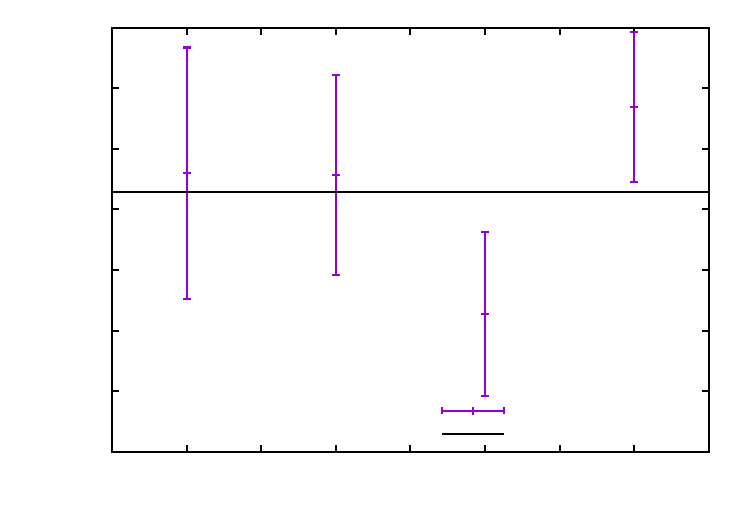
\includegraphics{gbesch}}%
    \gplfronttext
  \end{picture}%
\endgroup

	\caption{Berechnung der Erdbeschleunigung aus verschiedenen Periodendauern bei unterschiedlichen Seillängen und Mittelwert der Messungen.}
	\label{fig:gbesch}
\end{figure}

Lässt man es nun (nicht in der Nähe des Äquators) schwingen, so stellt man erstaunlicher Weise fest, dass das Pendel langsam seine Schwingungsebene dreht.
Dieser Effekt lässt sich durch die Corioliskraft erklären.
Diese ist eine Scheinkraft, welche dadurch ausgelöst wird, dass die Erde sich unter dem bewegenden Pendel wegdreht.

In der Voelesung hatten wir hergeleitet, dass die Periodendauer, mit welcher sich das Pendel einmal ganz um sich selbst dreht
\begin{align}
	T=\frac{2\pi}{\omega_r}=\frac{2\pi}{\omega\sin\phi}=\frac{24\si\hour}{\sin\phi}
\end{align}
beträgt.
Dabei gibt $\phi$ den Breitengrad des Standorts des Pendels.
Da $\sin\phi\leq1$ muss die Periodendauer $T\geq24\si\hour$ sein.
Wir hatten jedoch in $<+HIER BITTE WERTE EINTRAGEN+>\si\minute$ eine Umdrehung von $<+HIER BITTE WERTE EINTRAGEN+>\si\degree$, was einer Periodendauer von nur $<+HIER BITTE WERTE EINTRAGEN+>\si\hour$ entspricht.
Eine mögliche Erklärung ist, dass das Pendel nicht perfekt aufgehängt ist.
Es könnte also eine "`Vorzugsrichtung"' haben, in der es gerne schwingt.
Leider konnten wir dies nicht untersuchen, da es zu stark gedämpft war und wir nie bis in den entscheidenden Bereich gekommen sind.
Auch lag am Versuchstag der sogenannte Charron-Ring aufgrund der geringen Auslenkung nicht an.
Dieser soll Kräfte, welche seitlich auf das Pendel wirken durch Reibung unterdrücken.
Bei einer späteren Überprüfung mit stärkerer Auslenkung kamen wir auf bessere Werte, wenn auch nicht auf die rechnerischen.




\section{"`Fuß-GPS"'}
Das Funktionsprinzip von GPS kann man durch ein einfaches Experiment nachstellen:
Wenn drei Leute von bekannten Positonen aus zu einer vierten Person laufen, deren Ort unbekannt ist.
Die drei "`Photonen"' stoppen ihre Zeit, die sie benötigen, um zu der zu bestimmenden Stelle zu kommen.
Kennt man nun ihre ungefähre Geschwindigkeit und die Zeit, die sie um dem Start- zum Zielpunkt gebraucht haben, so kann man um den Startpunkt der einzelnen Personen Kreise ziehen.
Im Idealfall sollten sich alle drei Kreise an einem einzigen Punkt schneiden, welcher dann der Zielposition entspricht.
In der Realität wird dies nie erreicht werden, da die Personen nicht eine konstante Geschwindigkeit bei der Messung und bei der Geschwindigkeisbestimmung einhalten werden.

Übertragen auf das tatsächliche GPS bedeutet es, dass die Photonen sich zum Beispiel durch schwankende Ionosphären sich auch nicht konstant mit Lichtgeschwindigkeit fortbewegen.
Auch Streuung der Strahlung an der Umgebung kann zu störenden Einflüssen führen.
Die größte Unsicherheit besteht jedoch darin, dass das Empfangsgerät in der Regel keine Atomuhr hat, und so keine präzise Zeit messen kann.
Daher benötigt man nicht nur drei, sondern mindestens einen vierten Satelliten zur Positionsbestimmung.
Es gibt zwei Punkte, an denen sich der Empfänger befinden könnte, allerdings liegt der eine weit im Weltraum, so dass die Position auf der Erde doch wieder eindeutig ist.

Die Ergebnisse von unserem Versuch lassen sich auf dem Bild \ref{fig:gps} erkennen.
Dabei fällt auf, dass augenscheinlich alle Läufer bei der Messung zur Bestimmung der Geschwindigkeit etwas langsamer gegangen sind, als bei der tatsächlichen Messung.
Die tatsächliche Position der Zielperson liegt tatsächlich relativ genau zwischen den Kreisen.

\begin{figure}[h]
	\centering
	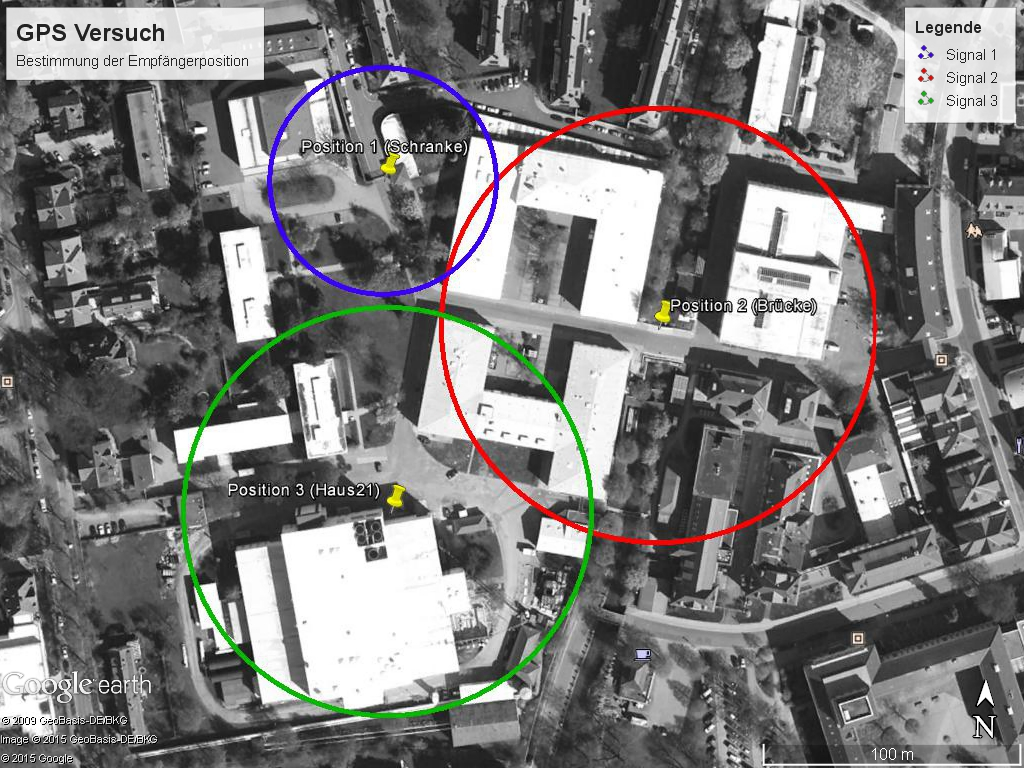
\includegraphics[scale=0.5]{GPS}
	\caption{Auftragung der Startpositionen der "`Photonen"', sowie der Entfernung, die sie jeweils zurückgelegt haben.}
	\label{fig:gps}
\end{figure}

\section{Bestimmung des Erdumfangs}
Schon Eratosthenes maß 200 v.Chr. den Umfang der Erde, als er bemerkte, dass genau zur Sonnenwende in Syene ein Brunnen keinen Schatten im inneren hatte.
Zur selben Zeit jedoch in Alexandria (ca. 790km nördlicher gelegen, aber nicht auf dem selben Längengrad, wesshalb die Luftlinie ca. 840km beträgt) warf ein Turm einen Schatten.
Wäre die Erde eine Scheibe, so wäre dies nicht möglich bei dem riesigen Abstand, den die Sonne zur Erde hat.
Er bestimmte nun die Entfernung mit Hilfe eines Sklaventrupps, der die Strecke abging und durch Lederriemen in der Schrittlänge begrenzt war.
Dadurch konnte die Entfernung in Längeneinheiten dieser Schritte angegeben werden.
Da jedoch nicht die Luftlinie interessant war und auch diese durch Hindernisse nicht direkt zu bestimmen war, mussten die Sklaven immer genau in Nord-Süd-Richtung oder Ost-West-Richtung laufen.

Aus Höhe des Turms und Länge des Schattens ließ sich der Winkel berechnen ($7^\circ11"$), der, wie in Abb. \ref{fig:umfang} zu sehen, so auch im Erdinneren zwischen den Orten vorhanden ist.
Daraus kann man herleiten, dass die 790km einem fünfzigstel des Erdumfangs entsprechen.









\bibliography{literatur}
\bibliographystyle{babalpha}
\end{document}
